\documentclass[12pt]{article}

\title{407 Problem Set 9}
\author{Alessandra Gudoy}
\date{November 2026}

\usepackage{graphicx} % Required for inserting images
\graphicspath{ {./images/} }
\usepackage{amssymb, amsmath, amsthm, xcolor}
\usepackage{multicol}

\usepackage{parskip}
\usepackage{changepage}
\usepackage[margin=1in]{geometry}
\usepackage[shortlabels]{enumitem}
\usepackage{setspace}

\newcommand{\head}{
    \vspace*{-2cm} % Or a larger value
    \null \hfill Alessandra Gudoy \\ 
    \null \hfill MATH 407: Numerical Analysis \\
    \null \hfill November 2026
}

\newcommand{\q}[1]{\textbf{#1}}
\newcommand{\R}{\mathbb{R}}

\definecolor{green}{HTML}{38761d}
\newcommand{\com}[1]{{\color{green}\%#1}}


\begin{document}

\head
\begin{center}
{\large Problem Set 9}
\end{center}

%--------------------%
%     Question 1     %
%--------------------%
\q{1.} We have the following to use to solve the system of linear equations:
\begin{align*}
    \begin{bmatrix}
        10  & 1 & 10 \\
        1  & 10 & 1 \\
        1  & 1 & 10
    \end{bmatrix}
    \begin{bmatrix}
        x_1 \\
        x_2 \\
        x_3
    \end{bmatrix}
    =
    \begin{bmatrix}
        12 \\
        12 \\
        12
    \end{bmatrix}.
\end{align*}

\textbf{Jacobi.}
We have $
    D^{-1} = 
    \begin{bmatrix}
        \frac{1}{10}  & 0 & 0 \\[1.5ex]
        0  & \frac{1}{10} & 0 \\[1.5ex]
        0  & 0 & \frac{1}{10}
    \end{bmatrix}.
$

Iteration \#1: Starting with $x_0 = \begin{bmatrix}0 \\ 0 \\ 0 \end{bmatrix}$,
\begin{align*}
    r_0 &= b - Ax_0
    = 
    \begin{bmatrix}
        12 \\[1.5ex]
        12 \\[1.5ex]
        12
    \end{bmatrix} - 
        \begin{bmatrix}
            10  & 1 & 10 \\[1.5ex]
            1  & 10 & 1 \\[1.5ex]
            1  & 1 & 10
        \end{bmatrix}
        \begin{bmatrix} 0 \\[1.5ex] 0 \\[1.5ex] 0 \end{bmatrix}
    =
    \begin{bmatrix}
        12 \\[1.5ex]
        12 \\[1.5ex]
        12
    \end{bmatrix}
\end{align*}
and
\begin{align*}
    x_1 = x_0 + D^{-1}r_0 
    =
    \begin{bmatrix}
        0 \\[1.5ex]
        0 \\[1.5ex]
        0
    \end{bmatrix} + 
        \begin{bmatrix}
            \frac{1}{10}  & 0 & 0 \\[1.5ex]
            0  & \frac{1}{10} & 0 \\[1.5ex]
            0  & 0 & \frac{1}{10}
        \end{bmatrix}
        \begin{bmatrix} 12 \\[1.5ex] 12 \\[1.5ex] 12 \end{bmatrix}
    =
    \begin{bmatrix}
        \frac{6}{5} \\[1.5ex]
        \frac{6}{5} \\[1.5ex]
        \frac{6}{5}
    \end{bmatrix}.
\end{align*}

Iteration \#2:
\begin{align*}
    r_1 &= b - Ax_1
    = 
    \begin{bmatrix}
        12 \\[1.5ex]
        12 \\[1.5ex]
        12
    \end{bmatrix} - 
        \begin{bmatrix}
            10  & 1 & 10 \\[1.5ex]
            1  & 10 & 1 \\[1.5ex]
            1  & 1 & 10
        \end{bmatrix}
        \begin{bmatrix} \frac{6}{5} \\[1.5ex] \frac{6}{5} \\[1.5ex] \frac{6}{5} \end{bmatrix}
    =
    \begin{bmatrix}
        12 - [10(\frac{6}{5}) + \frac{6}{5} + \frac{6}{5}] \\[1.5ex]
        \frac{12(5) - 60 - 6 - 6}{5} \\[1.5ex]
        -\frac{12}{5}
    \end{bmatrix}
\end{align*}
and
\begin{align*}
    x_2 = x_1 + D^{-1}r_1 
    =
    \begin{bmatrix} \frac{6}{5} \\[1.5ex] \frac{6}{5} \\[1.5ex] \frac{6}{5} \end{bmatrix} + 
        \begin{bmatrix}
            \frac{1}{10}  & 0 & 0 \\[1.5ex]
            0  & \frac{1}{10} & 0 \\[1.5ex]
            0  & 0 & \frac{1}{10}
        \end{bmatrix}
        \begin{bmatrix} -\frac{12}{5} \\[1.5ex] -\frac{12}{5} \\[1.5ex] -\frac{12}{5}
    \end{bmatrix}
    =
    \begin{bmatrix}
        \frac{6}{5} - \frac{1}{10}(\frac{12}{5}) \\[1.5ex]
        \frac{6}{5} - \frac{1}{5}(\frac{6}{5}) \\[1.5ex]
        \frac{6(5)-6}{25}
    \end{bmatrix}
    =
    \begin{bmatrix}
        \frac{24}{25} \\[1.5ex]
        \frac{24}{25} \\[1.5ex]
        \frac{24}{25}
    \end{bmatrix}.
\end{align*}

\newpage
\textbf{Gauss-Seidel.} Let $M = \begin{bmatrix} 10 & 0 & 0 \\ 1 & 10 & 0 \\ 1 & 1 & 10 \end{bmatrix}$ and $N = \begin{bmatrix} 0 & -1 & -1 \\ 0 & 0 & -1 \\ 0 & 0 & 0 \end{bmatrix}$ so that $A=M-N$.

We find $M^{-1}b$:
\begin{align*}
    My &= b \\
    \begin{bmatrix} 10 & 0 & 0 \\ 1 & 10 & 0 \\ 1 & 1 & 10 \end{bmatrix}
    \begin{bmatrix} y_1 \\ y_2 \\ y_3 \end{bmatrix} &=
    \begin{bmatrix} 12 \\ 12 \\ 12 \end{bmatrix} \\
    10y_1 = 12 &\quad\longrightarrow\quad y_1 = \frac{6}{5} \\[1.5ex]
    y_1 + 10y_2 = 12 &\quad\longrightarrow\quad y_2 = \frac{1}{10}(12 - \frac{6}{5}) = \frac{27}{25} \\[1.5ex]
    y_1 + y_2 + 10y_3 = 12 &\quad\longrightarrow\quad y_3 = \frac{1}{10}(12 - \frac{6}{5} - \frac{27}{25}) = \frac{243}{250} \\[1.5ex]
    M^{-1}b &= \begin{bmatrix} \frac{6}{5} \\[1.5ex] \frac{27}{25} \\[1.5ex] \frac{243}{250} \end{bmatrix}
\end{align*}

Now, we find $M^{-1}Nx_0$:
\begin{align*}
    Nx_0 = \begin{bmatrix} 0 & -1 & -1 \\ 0 & 0 & -1 \\ 0 & 0 & 0 \end{bmatrix} \begin{bmatrix} 0 \\ 0 \\ 0 \end{bmatrix} 
    = \begin{bmatrix} 0 \\ 0 \\ 0 \end{bmatrix}
\end{align*}

\begin{align*}
    My &= Nx_0 \\
    \begin{bmatrix} 10 & 0 & 0 \\ 1 & 10 & 0 \\ 1 & 1 & 10 \end{bmatrix} \begin{bmatrix} y_1 \\ y_2 \\ y_3 \end{bmatrix} &= \begin{bmatrix} 0 \\ 0 \\ 0 \end{bmatrix} \\
    \quad\longrightarrow\quad M^{-1}Nx_0 &= \begin{bmatrix} 0 \\ 0 \\ 0 \end{bmatrix}
\end{align*}
We get the following:
\begin{align*}
    x_1 &= M^{-1}Nx_0 + M^{-1}b
    = \begin{bmatrix} 0 \\[1.5ex] 0 \\[1.5ex] 0 \end{bmatrix} + \begin{bmatrix} \frac{6}{5} \\[1.5ex] \frac{27}{25} \\[1.5ex] \frac{243}{250} \end{bmatrix}
    = \begin{bmatrix} \frac{6}{5} \\[1.5ex] \frac{27}{25} \\[1.5ex] \frac{243}{250} \end{bmatrix}.
\end{align*}

\newpage
We know that $x=\begin{bmatrix} 1 \\ 1 \\ 1 \end{bmatrix}$, so we get the following errors.

\textbf{Iteration \#1 of Jacobi.}
\begin{align*}
    e_1 &= \begin{vmatrix}\begin{bmatrix} 1 \\[1.5ex] 1 \\[1.5ex] 1 \end{bmatrix} - 
    \begin{bmatrix}
        \frac{6}{5} \\[1.5ex]
        \frac{6}{5} \\[1.5ex]
        \frac{6}{5}
    \end{bmatrix} \end{vmatrix}
    = \begin{bmatrix}
        \frac{1}{5} \\[1.5ex]
        \frac{1}{5} \\[1.5ex]
        \frac{1}{5}
    \end{bmatrix} \\
    \longrightarrow ||e_1||_1 &= \sum_{k=1}^3 |x_k| = \frac{1}{5} + \frac{1}{5} + \frac{1}{5} = \frac{3}{5}
\end{align*}

\textbf{Iteration \#2 of Jacobi.}
\begin{align*}
    e_2 &= \begin{vmatrix}\begin{bmatrix} 1 \\[1.5ex] 1 \\[1.5ex] 1 \end{bmatrix} - 
    \begin{bmatrix}
        \frac{24}{25} \\[1.5ex]
        \frac{24}{25} \\[1.5ex]
        \frac{24}{25}
    \end{bmatrix} \end{vmatrix}
    = \begin{bmatrix}
        \frac{1}{25} \\[1.5ex]
        \frac{1}{25} \\[1.5ex]
        \frac{1}{25}
    \end{bmatrix} \\
    \longrightarrow ||e_2||_1 &= \sum_{k=1}^3 |x_k| = \frac{1}{25} + \frac{1}{25} + \frac{1}{25} = \frac{3}{25}
\end{align*}

\textbf{Iteration \#1 of Gauss-Seidel.}
\begin{align*}
    e_3 &= \begin{vmatrix}\begin{bmatrix} 1 \\[1.5ex] 1 \\[1.5ex] 1 \end{bmatrix} - 
    \begin{bmatrix}
        \frac{6}{5} \\[1.5ex]
        \frac{27}{25} \\[1.5ex]
        \frac{243}{250}
    \end{bmatrix} \end{vmatrix}
    = \begin{bmatrix}
        \frac{1}{5} \\[1.5ex]
        \frac{2}{25} \\[1.5ex]
        \frac{7}{250}
    \end{bmatrix} \\
    \longrightarrow ||e_3||_1 &= \sum_{k=1}^3 |x_k| = \frac{1}{5} + \frac{2}{25} + \frac{7}{250} = \frac{50+20+7}{250} = \frac{77}{250}
\end{align*}

%--------------------%
%     Question 2     %
%--------------------%
\newpage
\q{2.} (b) The Gauss-Seidel method took about 7.084980 seconds to run 8 iterations. The Jacobi method took about 0.270273 seconds to run 1361 iterations. MATLAB took 0.017995 seconds and my direct linear solve using LU factorization with partial pivoting took 0.765363 seconds.

The relative difference, in max-norm, between my solution using the Gauss-Seidel method and MATLAB's is about 0.00000541. The relative difference, in max-norm, between my solution using the Jacobi method and MATLAB's is about 0.00000030. The relative difference, in max-norm, between my solution using the direct linear solve and MATLAB's is about 0.00000000.

The Gauss-Seidel method took the longest, but ran much less iterations than the Jacobi method. The longer runtime can be explained by my repeated use of the LU Factorization function with partial pivoting in Gauss-Seidel where I did not use the vectorized approach, using a for-loop instead. Comparing it to the Jacobi method, the only major calculation taking time is $D^{-1}r$ to get the next iterate $x_{k+1} = x_k + D^{-1}r$. If I used the vectorized approach, the time it takes for the Gauss-Seidel to finish would be shorter, but still longer than Jacobi because of LU factorization.


%--------------------%
%     Question 3     %
%--------------------%
\q{3.} (c) The SteepestDescent() function took 3.626324 seconds and ran for 225033 iterations while the ConjugateGradient() function took 0.002529 seconds and ran for 90 iterations. Since we always just take the perpendicular path in SteepestDescent(), this can lead to more iterations whereas in ConjugateGradient() we account for previous directions to get the direction $p$ that points towards the true solution $x$.

Using the max-norm to find the relative differences, for Steepest Descent, it was about 0.00003642. For Conjugate Gradient, it was about 0.00000897.


%--------------------%
%     Question 4     %
%--------------------%
\newpage
\q{4.} As $n$ increase, the number of iterations also increases. Looking at the scatter plot, it seems to have a linear graph. For a small $n$, ConjugateGradient() took about $n$ iterations. However, as $n$ increased, it generally looks like it took about $\frac{1}{2}n$ iterations and decreased in the end. For example, when $A \in \R^{160\times160}$, it took 80 iterations which was exactly half, but when $A \in \R^{400\times400}$, it took 140 iterations.

\begin{figure}[h]
    \centering
    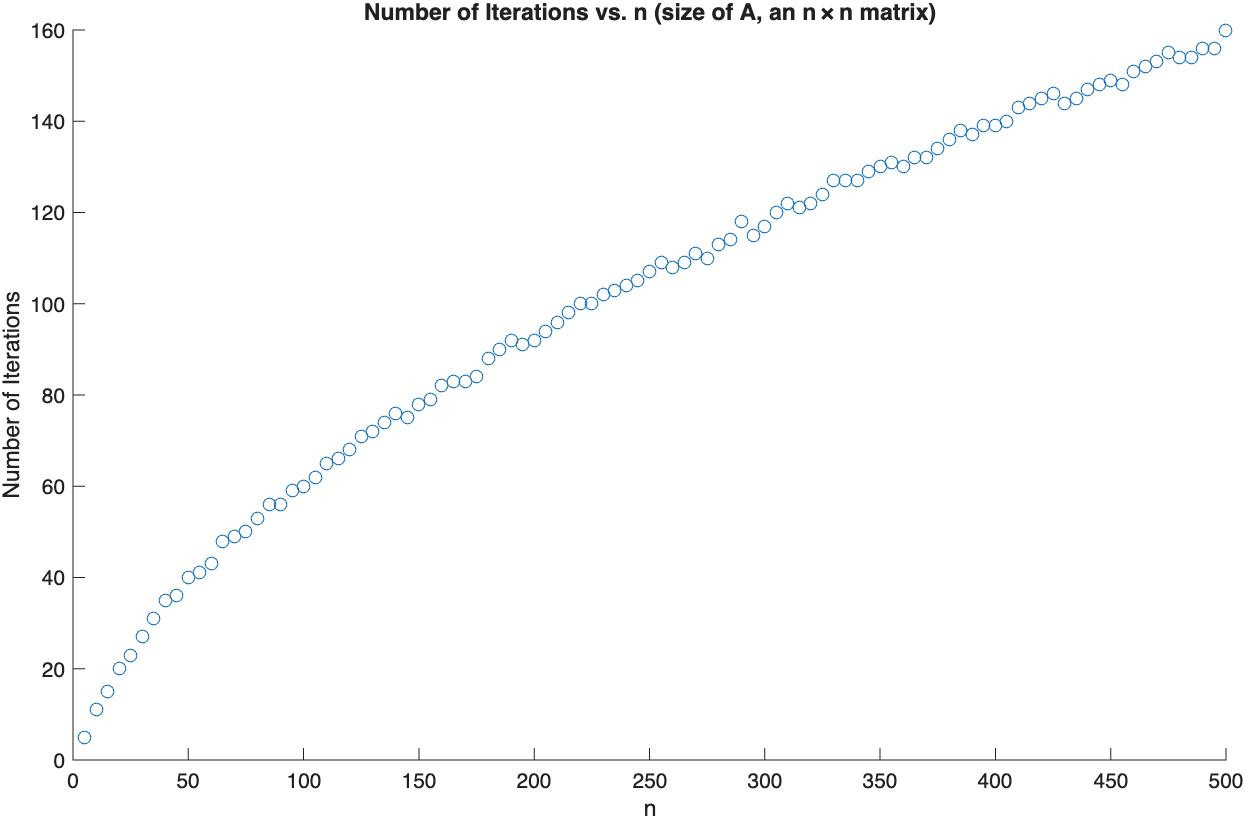
\includegraphics[width=0.75\textwidth]{ps9n4}
\end{figure}



%--------------------%
%     Question 5     %
%--------------------%
\q{5.} Using the ConjugateGradient() function with the stopping criteria in place, it did 159 iterations and had a relative difference of about $8.5923 \times 10^{-10}$. Using a modified function to run exactly 500 iterations, the relative difference was about $ 1.868310 \times 10^{-13}$, which is significantly closer to MATLAB's solution as Conjugate Gradient should arrive at the true solution $x$ after $n$ iterations for $A$ of size $n \times n$.

%--------------------%
%     Question 6     %
%--------------------%
\q{6.} Given the iterative scheme, we have
\begin{align*}
    \textbf{x}_{k+1} = \textbf{x}_k +\alpha(\textbf{b} - A\textbf{x}_k) &= (1-\alpha A)\textbf{x}_k + \alpha b \\
    &= M^{-1}Nx_k + M^{-1}b.
\end{align*}
Therefore, $M^{-1}N = 1-\alpha A$ and $M^{-1} = \alpha$. Substituting $M^{-1} = \alpha$ into the first equation, we get that $M^{-1}N = 1-\alpha A =M^{-1}\alpha = \alpha (\frac{1}{\alpha}-A)$, and $N=\frac{1}{\alpha}-A$ and $M=\frac{1}{\alpha}$.


\end{document}